\RequirePackage{lineno}
\documentclass[11pt,draft]{article}
\usepackage[final]{graphicx}
\usepackage{ucs,multicol,natbib,ifdraft,mathtools,xfrac,float,hyperref}
\usepackage[utf8x]{inputenc}
\usepackage[T1]{fontenc}
\usepackage[romanian]{babel}
\usepackage[a4paper,margin=2cm]{geometry}
\usepackage[printonlyused,withpage]{acronym}
\usepackage[usenames]{color}
\usepackage[obeyDraft,colorinlistoftodos]{todonotes}

\floatstyle{boxed}
\restylefloat{figure}

\graphicspath{ {./img/} }
\DeclareGraphicsExtensions{.pdf,.png,.jpg}

\presetkeys{todonotes}{inline}{}

\bibpunct{(}{)}{;}{a}{,}{,}
 
\makeatletter
\def\closeopenmulticols{%
   \def\@tempa{multicols}%
   \ifx\@tempa\@currenvir
      \end{multicols}%
  \fi 
}
\makeatother
\newcommand\Section[1]{%
 \closeopenmulticols
  \begin{multicols}{2}[\section{#1}]}


% close last open multicols
\AtEndDocument{ \closeopenmulticols}

\title{Studiu observațional asupra tratamentului incontinenței urinare de efort la pacientele din ambulator}
\author{Dr.~Andrei~Manu-Marin,~medic~primar~urologie\\Gnosis-EvoMed, str.~Suvenir,~nr.~10,~sect.~2,~București}
\date{}

\begin{document}

  \setlength{\columnsep}{25pt}
  \maketitle
  \ifdraft{ \linenumbers}{ }
  
 \todototoc
 \listoftodos

    \begin{abstract}
	\ac{IU} este definită ca orice pierdere involuntară a urinei. \ac{IU} face parte din categoria de simptome ale tractului urinar inferior (prescurtare: \ac{LUTS}) care includ dificultăți atât legate de stocarea urinei cât și de eliminarea ei, \ac{IU} fiind in categoria simptome de stocare. \ac{IU} poate fi caracterizată în plus prin datele obținute în urma anamnezei și a contextului simptomelor descrise de pacient. \todo{Mai multe detalii despre studiu}
  \end{abstract}
  
      \Section{Introducere}
	\ac{IU} este definită ca orice pierdere involuntară a urinei. \ac{IU} face parte din categoria de simptome ale tractului urinar inferior (prescurtat, \ac{LUTS}) care includ dificultăți atât legate de stocarea urinei cât și de eliminarea ei, \ac{IU} fiind in categoria simptome de stocare. \ac{IU} poate fi caracterizată în plus prin datele obținute în urma anamnezei și a contextului simptomelor descrise de pacient.  

	\ac{IUI} se definește ca pierderea de urină precedată de senzatia intensă de a urina, numită imperiozitate. \ac{IUE} se definește ca eliminarea involuntară de urină asociată cu anumite activități fizice (de ex. strănut și tuse). \ac{IUM} include caracteristici atât ale \ac{IUI} cât și ale \ac{IUE}. \todo{Informatii despre cercetare anterioara}
    
     \Section{Metode}
      \subsection{Protocolul clinic}
	Studiul este unul observational care evalueaza raspunsul unui grup de pacienti tratat ambulatoriu pe o perioada de 12 saptamani de tratament. Au fost inrolati 50 pacienti de ambele sexe(F=31,M=19) pe o perioada de 2 luni ($\pm$ 1 luna). Pacientii au efectuat proceduri de recuperare si stimulare periferica timp de 8 saptamani constand in 3 sesiuni de \ac{SEP} pe saptamana pentru 8 saptamani si 3 sesiuni de fizioterapie pe saptamana pentru 4 saptamani incepand din saptamana 5. Ulterior, pacientii au fost instruiti sa faca exercitii fizice acasa, fara supraveghere timp de 4 saptamani. O vizita de evaluare si urmarire a fost efectuata la 6 luni de la includerea in studiu.
      \subsection{Metode statistice}
	Pentru a analiza datele au fost folosite mai multe metode matematice bazate atat pe abordarea asa zis fregventionista cat si cea bayesiana. Datele au fost analizate folosind mediul de dezvoltare numit R (http://www.r-project.org/). Mai jos sunt prezentate pe scurt cateva dintre metode impreuna cu referinte bibliografice pentru mai multe detalii.
	\subsubsection{Testul Wilcoxon}
	Testul Wilcoxon este un test non-parametric pentru a testa ipoteza statistica de inegalitate a primului moment pentru doua populatii care se foloseste atunci cand distribuita celor 2 populatii nu este normala (alternativa pentru populatii normale este Testul Student t, sau Testul Z). Populatiile trebuie sa indeplineasca urmatoarele conditii:
	 \begin{itemize}
	 \item Datele exeminate provin din aceasi populatie
	 \item Datele sunt randomizate si independente
	 \item Datele sunt reprezentate prin numere intregi sau reale
	 \item Distributia este simetrica in jurul valorii medianei.
	 \end{itemize}
	Testul imperecheaza datele din cele 2 populatii $(x_{2,i},x_{1,i})$, elimina perechile de valori identice, si le sorteaza in ordinea crescatoare a diferentei absolute $|x_{2,i}-x_{1,i}|$ cu $R_i=1, ..., N_r$ semnificand rangul perechii $(x_{2,i},x_{1,i})$ dupa ordonare. Ulterior se calculeaza statistica $W = |\sum_{i=1}^{N_r} [sgn(x_{2,i} - x_{1,i}) \cdot R_i]| $ si un scor $p = \frac{W - 0.5}{\sigma_W}, \sigma_W = \sqrt{\frac{N_r(N_r + 1)(2N_r + 1)}{6}}$. Daca scorul este mai mare decat un prag conventional ales $0.05$ atunci ipoteza $H_0$ de egalitate a primului moment este rejectata. Pentru detalii vezi \citep{wilcoxon45,siegel56}.
    \Section{Rezultate}
    \subsection{Populatia}
    Un numar de 50 de pacienti au fost observati. Dintre acestia 62\% (N=31) sunt de sex feminin iar 38\% (N=19) sunt de sex masculin (proportia sexelor in grupa populatiei urbane cu varste cuprinse intre 27 si 83 ani la nivel national conform \citep{insee2011} este de 47\% M si 53\% F).
    Varsta pacientilor de sex feminin este distribuita normal in jurul mediei de 50 de ani si 7 luni ($\sigma=14.3,min=27,max=77$) iar cea a pacientilor de sex masculin este o combinatie de distributii normale centrate in jurul mediilor de 46 respectiv 75 ani ($\sigma_{1}=12.3 , \sigma_{2}=9.2,min=30,max=83$).
    %asTheEconomist(densityplot(~Varsta,data=IU,groups=Tip,auto.key=T,plot.points=F,main='',panel=function(...){
    %	panel.densityplot(...); #deseneaza graficul initial
    %	panel.xyplot(0:100,0.6*dnorm(0:110,46,12.3)+0.38*dnorm(0:110,75,9.2)) #deseneaza un kernel 
    %}))
    Pentru a evalua reprezentativitatea esantionului relativ la distributia varstelor in cadrul populatiei din Romania am apelat la datele oficiale din \citep{insee2011} care detaliaza numarul de cetateni romani pe sexe si categorie urban/rural pentru fiecare varsta la data de 1 iulie 2010. Analiza statistica s-a efectuat folosind testul Wilcoxon iar concluzia este ca atat esantionul de sex feminin ($p=0.005193$) cat si cel de sex masculin($p<2.2*10^{-16}$) corespund cu distributia generala in populatia urbana a Romaniei.
    \begin{figure}[H]
	\centering
	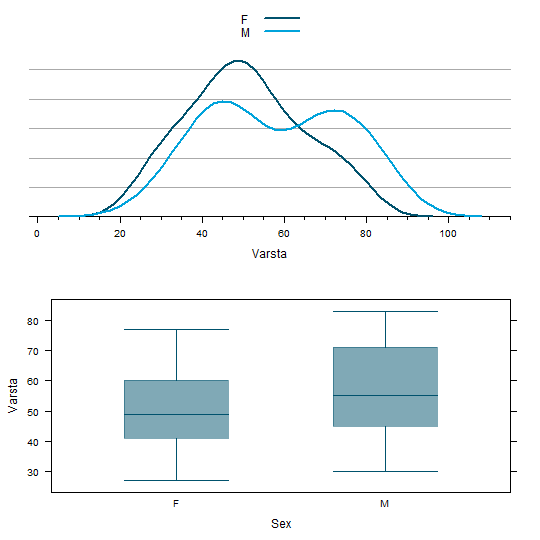
\includegraphics[width=0.8\linewidth]{incoVarstaSex}
	%dp1<-asTheEconomist(densityplot(~Varsta,data=IU,groups=Tip,auto.key=T,plot.points=F,main='',ylab=''))
	%dp2<-bwplot(Varsta~Tip,data=IU,ylab='',par.settings=theEconomist.theme())
	%dp1$yscale.components.old<-dp1$yscale.components
	%dp1$yscale.components<-function(...) { ret<-dp1$yscale.components.old(...); ret$left$labels$labels=NULL; ret}
	%print(dp1,split = c(1, 1, 1, 2))
	%print(dp2,split = c(1, 2, 1, 2),newpage=FALSE)
	\caption{Distributia sexelor participantilor la studiu}
	\label{fig:Distributia sexelor participantilor la studiu}
    \end{figure}
  Din punct de vedere al greutatii am evaluat indicatorul \ac{BMI} conform cu pragurile recomandate de \citep{whobmi06}. Astfel, pentru sexul feminin avem 13 persoane cu greutate normala ($BMI<25.0$, NOR), 16 supraponderale ($25.0 \geq BMI <30.0$, OVR) si 2 obeze($BMI \geq 30.0$, OBE). Pentru sexul masculin avem 3 persoane cu greutate normala, 12 supraponderale si 4 obeze.   
  \begin{table}[H]
  \centering
  \begin{tabular}{ |l|l|l|l| }
  \hline
  Sex & NOR & OVR & OBE \\ \hline
  F & 13 & 16 & 2 \\ \hline
  M & 3 &  12 & 4 \\ \hline
  \end{tabular}
  \caption{Numarul de persoane din fiecare categorie BMI pe sexe}
  \label{tab:BMIgSex}
\end{table}

    \begin{figure}[H]
	\centering
	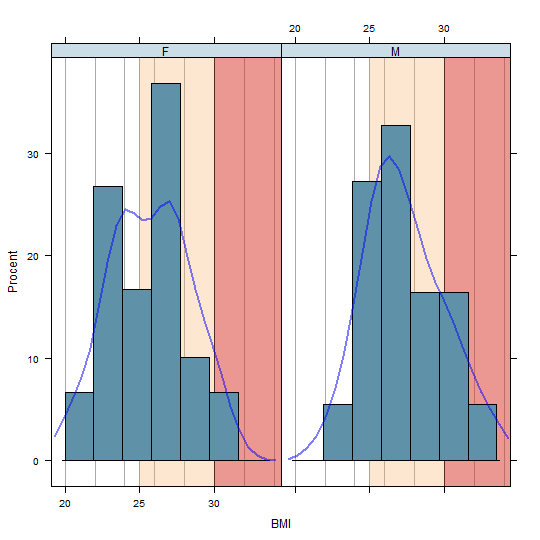
\includegraphics[width=0.8\linewidth]{incobmiDens}
	\caption{Distributia BMI pe sexe, Zona galbena marcheaza persoanele supraponderale si cea rosie pe cele obeze}
	\label{fig:incobmiDens}
    \end{figure}
  Distributia BMI pe grupa de varsta si pe sexe am evaluato la nivel national conform \citep{EHIS09} care ofera informatii detaliate despre incidenta problemelor de nutritie in randul tarilor memebre ale Uninii Europeene. Din cauza esantionului foarte mic, nu se poate trage concluzia ca populatia studiata este diferita de un esantion aleator la nivel national dar examinand graficul din figura alaturata se poate observa (cu exceptia unor situatii particulare - de exemplu toate persoanele de sex masculin din grupa de varsta 25-44 ani sunt supraponderale sau obeze) ca valorile procentelor urmaresc distributia nationala.
  \begin{figure}[H]
	\centering
	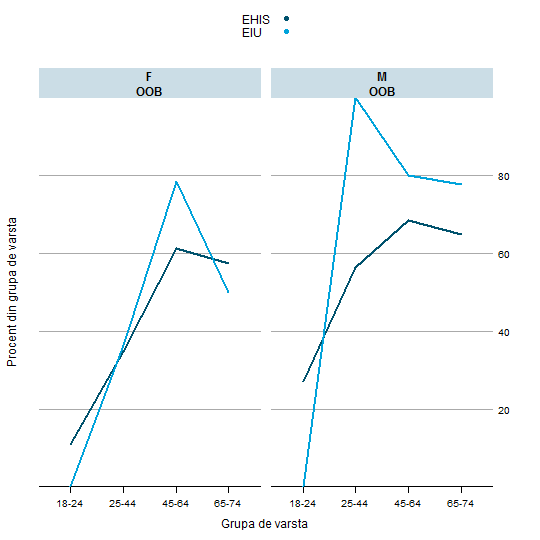
\includegraphics[width=0.8\linewidth]{incoBMIvsEHIS-OOB}
	\caption{Distributia procentului de persoane obeze in populatia studiata (EIU) si in populatia generala (EHIS) }
	\label{fig:incoBMIvsEHIS-OOB}
  \end{figure}
  
    \closeopenmulticols
    \begin{table}[H]
     \centering
    \begin{tabular}{ |l|l|l|l|l| }
     \hline
     Grupa de varsta & Sex & Categorie BMI & Numar persoane & Procent \\ \hline
    25-44 & F & NOR & 7  & 63.6 \\ \hline
    25-44 & F & OVR & 3  & 27.3 \\ \hline
    25-44 & F & OBE & 1  &  9.1 \\ \hline
    25-44 & M & NOR & 0  &  0.0 \\ \hline
    25-44 & M & OVR & 4  & 80.0 \\ \hline
    25-44 & M & OBE & 1  & 20.0 \\ \hline
    45-64 & F & NOR & 3  & 21.4 \\ \hline
    45-64 & F & OVR & 10 & 71.4 \\ \hline
    45-64 & F & OBE & 1  &  7.1 \\ \hline
    45-64 & M & NOR & 1  & 20.0 \\ \hline
    45-64 & M & OVR & 3  & 60.0 \\ \hline
    45-64 & M & OBE & 1  & 20.0 \\ \hline
    65-74 & F & NOR & 3  & 50.0 \\ \hline
    65-74 & F & OVR & 3  & 50.0 \\ \hline
    65-74 & F & OBE & 0  &  0.0 \\ \hline
    65-74 & M & NOR & 2  & 22.2 \\ \hline
    65-74 & M & OVR & 5  & 55.6 \\ \hline
    65-74 & M & OBE & 2  & 22.2 \\ \hline
    \end{tabular}
  \caption{Numarul de persoane si procentul din totalul de persoane dintr-o grupa de varsta din fiecare categorie BMI pe sexe si pe grupa de varsta}
  \label{tab:bmigCounts}
 \end{table}
  \begin{multicols}{2}
 Studiul a inregistrat si  date referitor la comorbiditatea 

        \closeopenmulticols
  \bibliographystyle{plainnat}
  \bibliography{incoStudy}
  
  \section*{Glosar}
  \begin{acronym}[LUTS]
    \acro{IU}{Incontinența Urinară}
    \acro{IUI}{Incontinența Urinară prin Imperiozitate}
    \acro{IUE}{Incontinența Urinară de Efort}
    \acro{IUM}{Incontinența Urinară Mixtă}
    \acro{LUTS}{Lower Urinary Tract Symptoms}
    \acro{SEP}{Stimulare Electrica Periferica}
    \acro{BMI}{Body-Mass Index}
  \end{acronym}
 
 \listoffigures
 \listoftables
   
\end{document}
